\begin{figure}[H]
    \centering
    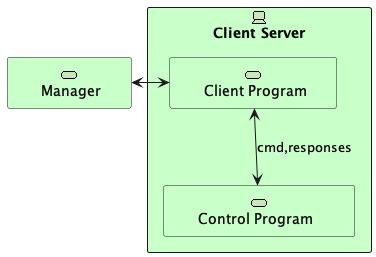
\includegraphics[height=0.2\textheight]{./part/Proyecto_ejecutivo/memoria_descriptiva/descripcionDelProyecto/client/uml/clientServerConcept}
    \caption{Diagrama UML de despliegue del cliente}\label{fig:Diagrama UML de despliegue del cliente}
\end{figure}

\subparagraph{Dominio}

Hay que tener en cuenta que en este programa será casi todo infrestructura. ya que una vez recepcionado el comando mediante el RPC
solo habrá que ejecutarlo en el servidor cliente y será tarea del cliente configurar dicho servidor para que dicho comando exista. Será tarea del programa a ejecutar interpretar dicho comando y trasnformar ese comando y esos argumentos en un dominio interno. Por ejemplo un programa típico de consola en un sistema UNIX

\begin{verbatim}
    ./runMyComand --arg=arg1 --argN=argN
\end{verbatim}


Las posibilidades son tantas como comandos haya instalados en el servidor cliente. En nuestro caso podremos mandar a ejecutar todos los comandos que queramos que vengan previamente instalados en un sistema UNIX y además el programa de control donde podremos interactuar con el motor de corriente continua

\begin{verbatim}
    ./pidControl --velocity=30rpm
    ./pidControl --position=180deg
    ./pidControl --setP=1
    ./pidControl --setI=0
    ./pidControl --setD=0
    ./pidControl --enabled=true
    ./pidControl --enabled=false
\end{verbatim}

aquí podemos ver por ejemplo los comándos básicos de un control pid que podremos ejecutar. En la descripción del programa de control y su dominio lo veremos en más detalle


\begin{figure}[H]
    \centering
    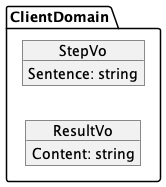
\includegraphics[height=0.2\textheight]{./part/Proyecto_ejecutivo/memoria_descriptiva/descripcionDelProyecto/client/uml/clientDomain}
    \caption{Diagrama UML de el dominio de cliente}\label{fig:Diagrama UML de el dominio de cliente}
\end{figure}

\begin{itemize}
    \item StepDomain
    \begin{itemize}
        \item StepVo
    \end{itemize}
    \item ResultDomain
    \begin{itemize}
        \item ResultVo
    \end{itemize}
\end{itemize}

\subparagraph{casos de uso}

Vamos a describir los casos de uso que podrán ejecutarse en el programa client. En este caso no tendremos Entities porque no necesitamos identificadores.
Tendremos los Value Objects para los steps que nos llegaran a modo de request y el necesario para responder. En este sistema no hay persistencia.

\textbf{Execute Unary Step}

Centrando en un caso de uso de este tipo de steps en nuestro programa de control sirve por ejemplo para establecer un parámetro de control del PID. Cualquiera de los siguientes.
\begin{verbatim}
    ./pidControl --velocity=30rpm
\end{verbatim}

Podemos ver en~\ref{fig:Use Case-Execute Unary Step} el diagrama de flujo que responde a este caso de uso

\begin{figure}[H]
    \centering
    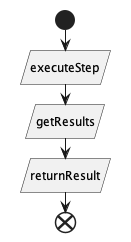
\includegraphics[height=0.2\textheight]{./part/Proyecto_ejecutivo/memoria_descriptiva/descripcionDelProyecto/client/uml/executeUnaryStep}
    \caption{Use Case: Execute Unary Step}\label{fig:Use Case-Execute Unary Step}
\end{figure}

\textbf{Execute ClientStream Step}

Centrando en un caso de uso de este tipo de steps en nuestro programa de control sirve por ejemplo para establecer una configuración completa con una sola llamada para nuestro PID:
\begin{verbatim}
    ./pidControl --velocity=30rpm
    ./pidControl --position=180deg
    ./pidControl --setP=1
    ./pidControl --setI=0
    ./pidControl --setD=0
\end{verbatim}

Podemos ver en~\ref{fig:Use Case-Execute ClientStream Step} el diagrama de flujo que responde a este caso de uso

\begin{figure}[H]
    \centering
    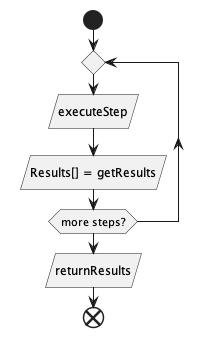
\includegraphics[height=0.2\textheight]{./part/Proyecto_ejecutivo/memoria_descriptiva/descripcionDelProyecto/client/uml/executeClientStreamStep}
    \caption{Use Case: Execute ClientStream Step}\label{fig:Use Case-Execute ClientStream Step}
\end{figure}

\textbf{Execute ServerStream Step}

Centrando en un caso de uso de este tipo de steps en nuestro programa de control sirve por ejemplo para habilitar el control del pid durante un determinado tiempo e ir devolviendo el estado la variable de control
\begin{verbatim}
    ./pidControl --enabled=true --time=10s
\end{verbatim}

O dejar el control activado indefinidamente hasta que llege otra request de tipo Unary que lo detenga

\begin{verbatim}
    ./pidControl --enabled=false
\end{verbatim}

Podemos ver en~\ref{fig:Use Case-Execute ServerStream Step} el diagrama de flujo que responde a este caso de uso

\begin{figure}[H]
    \centering
    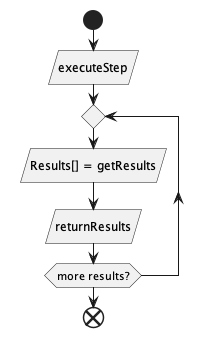
\includegraphics[height=0.2\textheight]{./part/Proyecto_ejecutivo/memoria_descriptiva/descripcionDelProyecto/client/uml/executeServerStreamStep}
    \caption{Use Case: Execute ServerStream Step}\label{fig:Use Case-Execute ServerStream Step}
\end{figure}

\textbf{Execute Bidirectional Step}

Usando el ejemplo anterior, si no queremos habilitar el control indefinidamente y deshabilitarlo mediante otra request podemos usar este caso de uso.

\begin{verbatim}
    ./pidControl --enabled=true --time=10s
\end{verbatim}

y posteriormente cuando el Cliente decida.

\begin{verbatim}
    ./pidControl --enabled=false
\end{verbatim}

Este caso de uso es el que utilizaremos para el control manual.

Podemos ver en~\ref{fig:Use Case-Execute Bidirectional Step} el diagrama de flujo que responde a este caso de uso

\begin{figure}[H]
    \centering
    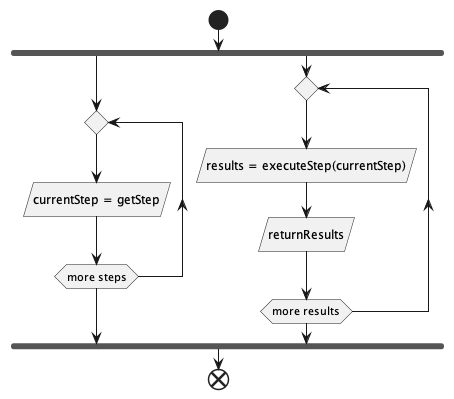
\includegraphics[height=0.2\textheight]{./part/Proyecto_ejecutivo/memoria_descriptiva/descripcionDelProyecto/client/uml/executeBidiStep}
    \caption{Use Case: Execute Bidirectional Step}\label{fig:Use Case-Execute Bidirectional Step}
\end{figure}

\subparagraph{estructura de carpetas}

En el proyecto constará de 4 carpetas principales

\tiny
\dirtree{%
    .1 Project .
        .2 Domain.
        .2 Application.
        .2 Adapter.
        .2 Bootstrap.
}
\normalsize

\textbf{Dominio}

\begin{figure}[H]
    \tiny
\dirtree{%
    .1 Domain.
        .2 Step.
            .3 StepVo.
            .3 Repository.
                .4 consoleWrite.
            .3 Services.
                .4 Executor.
        .2 Result.
            .3 ResultVo.
}
\normalsize
    \caption[Diagrama de objetos de dominio]{}\label{fig:1-ClientDomainFolderStructure}
\end{figure}

\textbf{Aplicación}

\tiny
\dirtree{%
.1 Application.
    .2 Port.
        .3 in.
            .4 Step.
                .5 Execute.
                    .6 Command.
                    .6 UseCase.
}
\normalsize

\textbf{Adapters}

\tiny
\dirtree{%
    .1 Adapter.
        .2 in.
            .3 GRPC.
                .4 Harán uso de los useCases de aplicación cuando llegue una request RPC.
            .3 Console.
                .4 Por ejemplo si quisieramos ejecutar los casos de uso mediante terminal.
        .2 out.
            .3 console.
                .4 implementación de los repository de llamada a los servidores clientes.
}
\normalsize





